\section{Nebulas Asset Supervision}

\label{supervision}

As show in Figure~\ref{fig:assets}, Nebulas assets include two parts: Community public assets and Nebulas Foundation assets.

\subsection{Community public assets}

\subsubsection{Composition}

\begin{itemize}
	\item 35,000,000 NAS (35\% of total circulation): community reserved assets as stated in the \textit{Nebulas Non-technical Whitepaper}
    \item 8,219.1744 NAS/Day: from consensus/block generation issuance, includes:
	    \begin{itemize}
			\item 2\%: Consensus/block generation issuance
			\item 1\%: Nebulas Council Project Development Fund reserve
		\end{itemize}
	\item 1\%(initial): Native incentive for Developer Incentive Protocol (DIP)~\cite{mauvepaper}, since May 13, 2019
\end{itemize}

\subsubsection{Supervision}

Public assets belong to the Nebulas community; they are automatically distributed and managed via the on-chain governance process and is overseen by the Nebulas Council.

\subsection{Nebulas Foundation assets}

\subsubsection{Composition}

\begin{itemize}
	\item 20,000,000 NAS (20\%): Nebulas team reserved as stated in the \textit{Nebulas Non-technical Whitepaper}
    \item 5,000,000 NAS (5\%): Nebulas Community Development Fund (Eco-investment Balance)
	\item Early private equity project development funds
	\item Early ecological investment income
\end{itemize}

\subsubsection{Supervision}

The Nebulas Foundation assets are managed by the Nebulas Foundation. The Foundation shall ensure that the use of asset information is open and transparent.

\begin{figure}
	\centering
	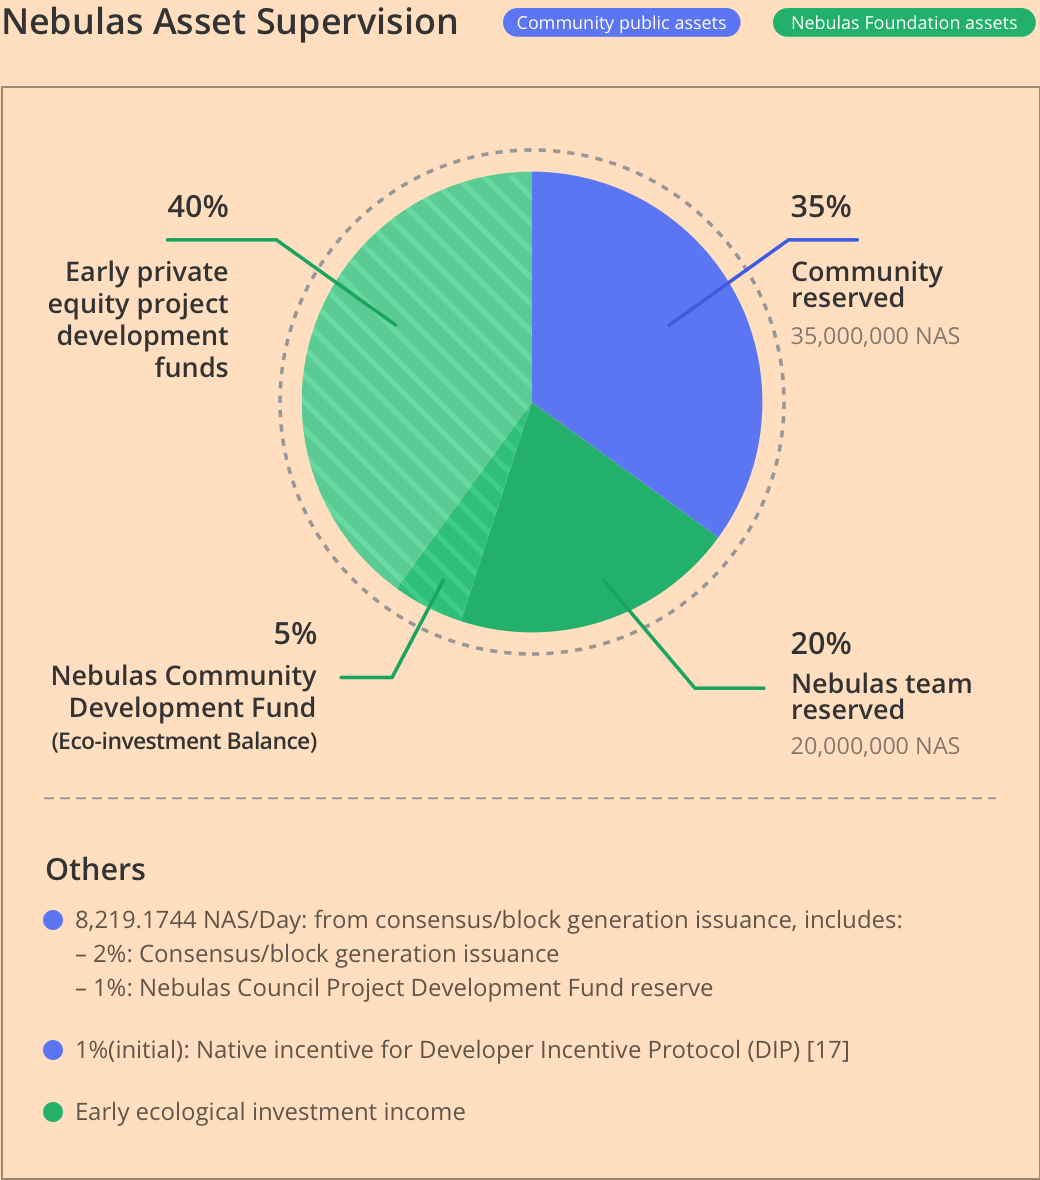
\includegraphics[width=1\textwidth]{../common/en/assets.png}
	\caption{Nebulas Assets Supervision \label{fig:assets}}
\end{figure}